\chapter{Supply Chain Management}
In dem nachfolgendem Kapitel wird zuerst der Begriff Supply Chain Management genauer definiert. Danach werden die Gründe für Entwicklung eines Supply Chain Management genannt sowie die Ziele und dessen Nutzen aufgezeigt.

\section{Begriffsdefinition Supply Chain Managment}
Um den Begriff des Supply Chain Managements zu verstehen, muss erst einmal die Bezeichnung der Supply Chain (zu dt. Lieferkette) genauer angeschaut werden.
Das Konzept der Lieferkette gehört zu den wichtigsten Bestandteilen der Wirtschaftswissenschaften.

\begin{figure}[h]
	\centering
	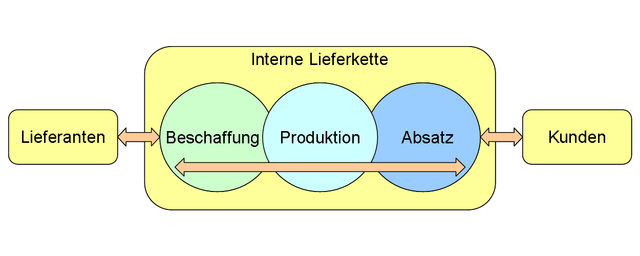
\includegraphics[width=0.6\textwidth]{../pics/Lieferkette}
\end{figure}

\section{Das SCM Haus}
Um die zahlreichen Facetten von Supply Chain Management aufzuzeigen, werden die einzelnen Elemente in einem Haus zusammen gefasst.

Um ein stabiles Haus bauen zu können, wird starkes Fundament benötigt. In unserem Fall bestehen die Grundmauern aus den verschiedensten Abteilungen, Aufgaben und Prozesse im gesamtem Unternehmen.
